\section{Искуственные нейронные сети}

\indent
\indent
Настоящая часть работы предназначена для читателя, не знакомого с 
искуственными нейронными сетями. Здесь будут приведены теоретические 
основы глубокого обучения и рассмотрены сверточные архитектуры, 
используемые в дальнейшей работе.

\subsection{Базовая информация о глубоком обучении}

\indent
\indent
Начнем с рассмотрения одиночного нейрона
 --- перцептрона Розенблатта --- базового элемента, содержащегося в большинстве современных нейросетевых архитектур.
Перцептрон имеет несколько входов и один выход, значение на котором
вычисляется как взвешенная сумма значений входов 
(рисунок \ref{tikzpicture: perceptron}).
Кроме того, обычно
к выходному значению применяется сдвиг и некоторая нелинейная функция, 
называющаяся функцией активации нейрона. Ее предназначение мы обсудим позже.

\begin{figure}[h!]
    \begin{center}
   	    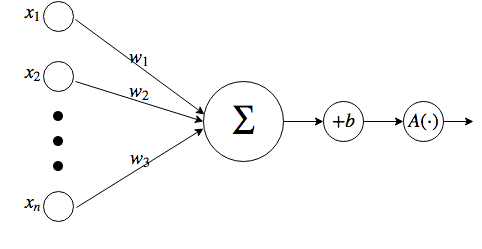
\includegraphics[width=0.6\linewidth]{Perceptron}
   	\end{center}
   	\caption{Схематическое изображение работы одного отдельного нейрона.}
   	\label{tikzpicture: perceptron}
\end{figure}


\indent
\indent
Таким образом, значение на выходе нейрона задается
 выражением \ref{eq:perceptron}.

\begin{equation}\label{eq:perceptron}
    f(\vec{x}) = S(\sum_{i=1}^n x_i w_i + b)
\end{equation}


где $f(\vec{x})$ -- выходное значения нейрона, посчитанное для входов $x_i$,
$w_i$ -- весовые коэффициенты для входов, $b$ -- параметр смещения, 
а $S$ --- нелинейная функция активации. Далее для упрощения повествования
положим $b \equiv 0$.

\indent
\indent
Существуют множество различных функций активации, например, гиперболический
тангенс, логистическая сигмоида или \textit{ReLU}. Перечисленные
функции особенно популярны, так как значения их производных простым образом 
выражаются через значения самой функции (выражение \ref{eq:activations}), 
что, как будет показано далее, позволяет
ускорить процесс обучения нейросети.


\begin{equation}\label{eq:activations}
	\begin{gathered}
	    S(x) = th(x) = \frac{e^x - e^{-x}}{e^x + e^{-x}},    \;   th’(x) = 1 - th(x)^2   \\    
	    S(x) = \sigma(x) = \frac{1}{1 + e^{-x}},   \;   \sigma’(x) = \sigma(x)(1 - \sigma(x)) \\
	    S(x) = ReLU = max(0, x),   \;   ReLU’(x) = \theta(x)
	\end{gathered}
\end{equation}
где $\theta(x)$ -- функция Хэвисайда.


\indent
Одиночный нейрон не способен выразить сложные в наборе
признаков $\vec{x}$, поэтому нейроны объединяют в слои, а их, в свою 
очередь, в многослойные нейросети . Рассмотрим нейронную сеть,
состоящую из двух слоев. Пусть количество количество входных признаков
равно $N$, количество нейронов скрытого слоя $P$,
а размер выхода -- $M$, рисунок \ref{tikzpicture: fc_net}.
 
\begin{figure}[h!]
    \begin{center}
   	    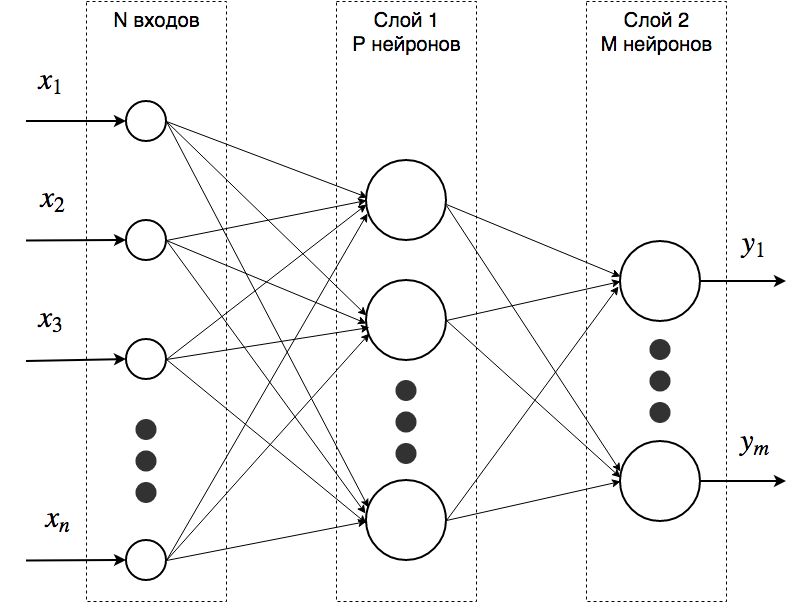
\includegraphics[width=0.9\linewidth]{FC_net}
   	\end{center}
   	\caption{Схематическое изображение полносвязной нейронной сети.}
   	\label{tikzpicture: fc_net}
\end{figure}

Рассмотрев выражение \ref{eq:perceptron} можно увидеть, что 
совокупность значений нейронов на 1 слое может быть получена 
простым матричным умножением входов $\vec{x}$ на весовую матрицу
 $W^1$ размера $P \times N$, с последующим поэлементным применением 
функции активации к получившися значениям. Аналогично, значения нейронов
2 слоя получаются умножением предыдущих значений на весовую матрицу
$W^2$ размером $M \times P$. Таким образом, применение нейросети
ко входу $\vec{x}$ можно задать выражением \ref{eq:forward}.

\begin{equation}\label{eq:forward}
	   \vec{y} = W^{2} S(W^{1} \vec{x})
\end{equation}
где $S(\cdot)$ -- применение нелинейности к каждому элементу входного 
вектора.

Близость предсказания сети к правильным ответам оценивается
с помощью функции потерь \textit{(loss function)}. В самом простом виде
это может быть сумма разностей между выходами сети и правильными ответами,
выражение \ref{eq:loss}.

\begin{equation}\label{eq:loss}
	   L(\vec{x}) = sum(\vec{y_{gt}} - \vec{y}) = sum(\vec{y_{gt}} - W^{2} S(W^{1} \vec{x}))
\end{equation}

% https://habr.com/ru/company/ods/blog/344116/
% https://ru.wikipedia.org/wiki/Метод_обратного_распространения_ошибки
 
 
\subsection{Сверточные нейронные сети}
\indent
\indent
Сверточная неройнная сеть --- это специальная сеть, сконструированная для 
обработки изображений, хотя в настоящее время спектр их применения 
значительно расширился. Как следует из названия, основной таких сетей 
являются сверточные слои \textit{convolutional layers}. 
Кроме того, вместе с ними используются такие
слои как \textit{BatchNormalization}, \textit{Pooling}, \textit{Softmax} и \textit{Dropout}.

\indent
\indent
Рассмотрим, как устроено применение оператора свертки к изображению.
% https://habr.com/ru/company/ods/blog/344008/

\subsection{Используемые архитектуры}
В данное работе в качестве базовой неросетевой архитектуры используется
ResNet \cite{resnet}.
